\chapter{Zanarkand}
\begin{enumerate}
    \item \sd, \cs[0:50], walk left. \fmv+\cs[2:20]
    \item Move left to the sphere, \sd, \cs[1:40]. Walk further left and follow the path down, \cs[3:20], walk left onto the next screen.
    \item \textit{If \rikku\ doesn't have \od} \formation{\tidus}{\auron}{\rikku}, otherwise \formation{\tidus}{\auron}{\kimahri}
    \item You can charge \rikku's \od\ on an encounter with a Behemoth or a Defender Z (Escape with the others).
    \item Open the first chest on the left for the \textbf{Fortune Sphere}, continue on the path until you get inside the Dome.
    \item If you got \textbf{4 Return Spheres} and you missed the Overkill on \textbf{Seymour Flux} kill two \textbf{YKT-11} or one \textbf{Defender Z} with \formation{\tidus}{\auron}{\yuna}, only \yuna\ needs the AP.
\end{enumerate}
\begin{encounters}
    \begin{itemize}
        \item YKT-11:
            \begin{itemize}
                \yunaf Attack
                \tidusf Attack
                \item Flee
            \end{itemize}
        \item Defender Z:
            \begin{itemize}
                \summon{\bahamut}
                \bahamutf Attack
            \end{itemize}
    \end{itemize}
\end{encounters}
\begin{enumerate}[resume]
    \item After Seymour's Mom \cs, if you had \textbf{4 Return Sheres} \pickup{Friend Sphere} on the right path.
    \item When you leave the last encounter zone, the hallway before the Zanarkand Trials, \pickup{Luck Sphere} on the right.
\end{enumerate}
\bothvfill
\bothnp
\winvfill
\winnp
\lossvfill
\lossnp
\begin{spheregrid}
    \begin{itemize}
        \yunaf
        \begin{itemize}
            \item \textit{If you got \textbf{4 Return Spheres}:}
                \begin{itemize}
                    \item Friend Sphere to \lulu\ $\downarrow\downarrow$
                    \item Luck Sphere, Fortune Sphere
                    \item Str+4, Str+4
                    \item Move to the empty node between HP+200 and Agi+4 #TODO
                    \item Agi+4
                    \item Return to the Agi+4 node you just activated
                    \item Str+3
                    \item Return to the Str+3 node you just activated
                    \item Agi+4
                \end{itemize}
            \ifthenelse{\equal{\colstyle}{multi}}{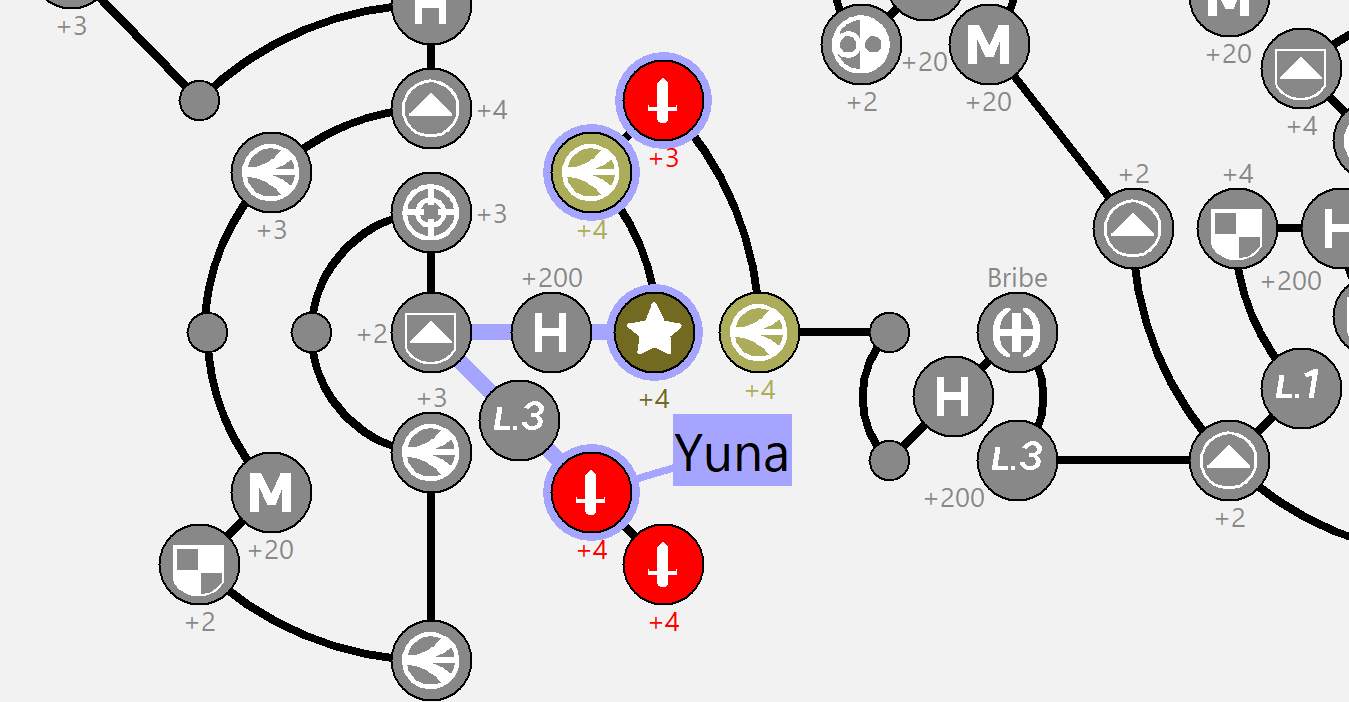
\includegraphics[width=.5\columnwidth]{graphics/4_returns_w_luck_pt1}}{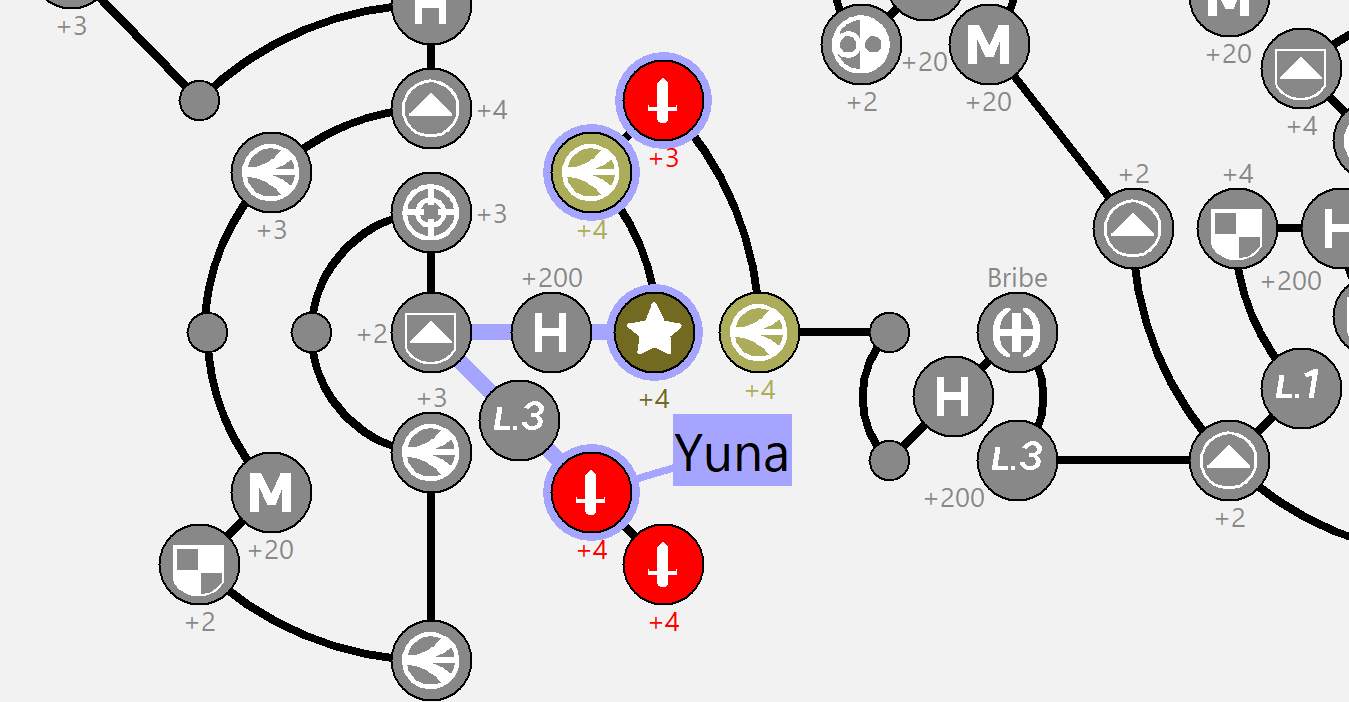
\includegraphics[width=.2\columnwidth]{graphics/4_returns_w_luck_pt1}}
            \item \textit{If you got \textbf{2 Return Spheres}:}
                \begin{itemize}
                    \item Use Blk Mag Sphere on Fire
                    \item Return Sphere to Fire
                    \item Move $\leftarrow\leftarrow\leftarrow$
                    \item Luck Sphere, Fortune Sphere
                    \item Agi+4
                    \item Move $\leftarrow\leftarrow\leftarrow$ #TODO
                    \item MP+20, Str+2
                \end{itemize}
            \ifthenelse{\equal{\colstyle}{multi}}{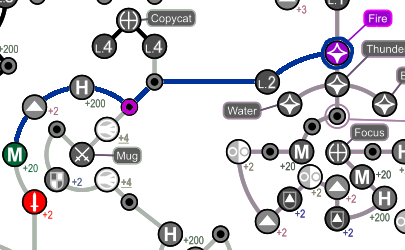
\includegraphics[width=.5\columnwidth]{graphics/2_and_2_with_luck}}{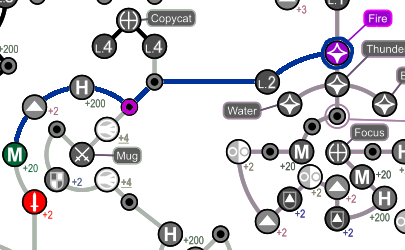
\includegraphics[width=.2\columnwidth]{graphics/2_and_2_with_luck}}
            \item \textit{If you got \textbf{0 Return Spheres}:}
                \begin{itemize}
                    \item Move $\swarrow\swarrow$
                    \item Luck Sphere, Fortune Sphere, Spare Change
                \end{itemize}
            \ifthenelse{\equal{\colstyle}{multi}}{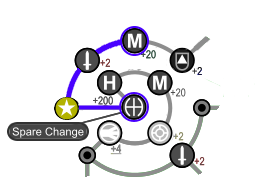
\includegraphics[width=.7\columnwidth]{graphics/0_return_w_luck}}{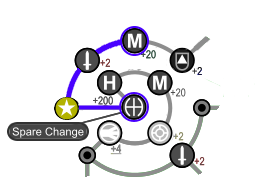
\includegraphics[width=.25\columnwidth]{graphics/0_return_w_luck}}
        \end{itemize}
    \end{itemize}
\end{spheregrid}
\bothcb \wincb \losscb
\begin{enumerate}[resume]
    \item \formation{\tidus}{\auron}{\yuna}
    \item \textit{If you had 0 Return Spheres:}
        \begin{itemize}
            \item Customize:
                \begin{itemize}
                    \auronf Shimmering Blade $\rightarrow$ First Strike
                    \yunaf Staff $\rightarrow$ First Strike
                \end{itemize}
        \end{itemize}
\end{enumerate}
\begin{enumerate}[resume]
    \item {\large \save}
\end{enumerate}
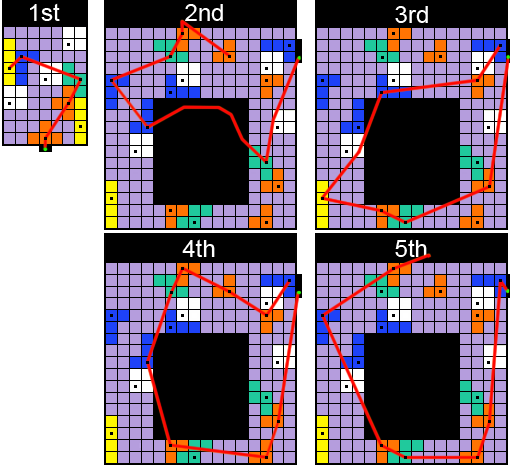
\includegraphics[width=.95\columnwidth]{graphics/Zanarkand_Trials}
\begin{enumerate}[resume]
    \item Push in the pedestals starting from the Top Left, to Bottom Left, then Top Right, Bottom Right, then Besaid Sphere. After pushing in each pedestal, do the corresponding puzzle, shown above.
    \item After the second puzzle, take the Kilika Sphere on the left and put it into the second pedestal.
    \item After the fifth puzzle, take the Besaid Sphere from the right and put it into the fifth pedestal.
    \item \cs, run into the large room
\end{enumerate}
\begin{battle}[52000]{Spectral Keeper}
    \begin{itemize}
        \summon{\bahamut}
        \bahamutf Attack x2
    \end{itemize}
\end{battle}
\bothvfill\winvfill\lossvfill
\begin{spheregrid}
    \begin{itemize}
        \item \textit{If you had 4 \textbf{Return Spheres}}:
            \begin{itemize}
                \item Use Blk Mag Sphere on Fire
                \item Return Sphere to Fire
                \item Move $\leftarrow\leftarrow\leftarrow$
                \item Luck Sphere, Fortune Sphere
                \item Agi+4
                \item Move $\leftarrow\leftarrow\leftarrow$ #TODO
                \item MP+20, Str+2
            \end{itemize}
    \end{itemize}
    \ifthenelse{\equal{\colstyle}{multi}}{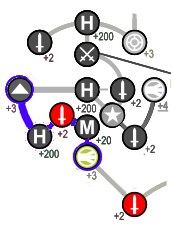
\includegraphics[width=.5\columnwidth]{graphics/4_return_before_yunalesca}}{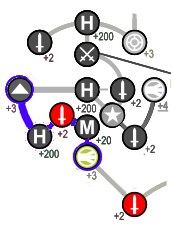
\includegraphics[width=.25\columnwidth]{graphics/4_return_before_yunalesca}}
\end{spheregrid}
\begin{enumerate}[resume]
    \item \save, Run up, \sd\ by mashing another button (like \textbf{R1}) at the same time as confirm, walk up to Yunalesca's room, \sd
\end{enumerate}
\begin{battle}[132000]{Yunalesca}
    \begin{itemize}
        \summon{\bahamut}
        \bahamutf Attack x3
    \end{itemize}
    If any weapon drops, it will have \textbf{Zombie Strike}
\end{battle}
\begin{enumerate}[resume]
    \item \sd, leave room, walk down steps, \sd, go down on the next screens, \save, go up the lift, walk out of the cloister of trials, walk down the steps, walk down, \sd\ during \cs+\skippablefmv
\end{enumerate}